% sezione XML frame 01
\begin{frame}
	\frametitle{Codifica ad alto livello}
	\framesubtitle{Sistemi di marcatura}
	\addtocounter{nframe}{1}

	\begin{block}{Metodi e tecniche per la codifica di testi}
		La riflessione sui metodi e le pratiche migliori per la codifica elettronica dei testi è stato uno dei temi fondamentali della ricerca e della sperimentazione nel dominio dell’Informatica umanistica per molti anni.
	\end{block}

\end{frame}

% sezione XML frame 02
\begin{frame}
	\frametitle{Markup language e XML}
	\framesubtitle{soluzione corrente per la codifica dei testi}
	\addtocounter{nframe}{1}

	\begin{block}{XML per la descrizione e la codifica}
		Ad oggi la soluzione considerata ottimale per una corretta rappresentazione del testo è l'adozione dei markup language descrittivi basati su XML.
	\end{block}

	\begin{block}{TEI-XML}
		Standard de facto per la codifica dei testi è considerato lo schema XML messo a punto dalla Text Encoding Initiative (TEI-XML).
	\end{block}

\end{frame}

% sezione XML frame 02b
\begin{frame}
	\frametitle{Lo schema TEI-XML}
	\framesubtitle{Estratto di documento TEI-XML}
	\addtocounter{nframe}{1}

	\begin{center}
		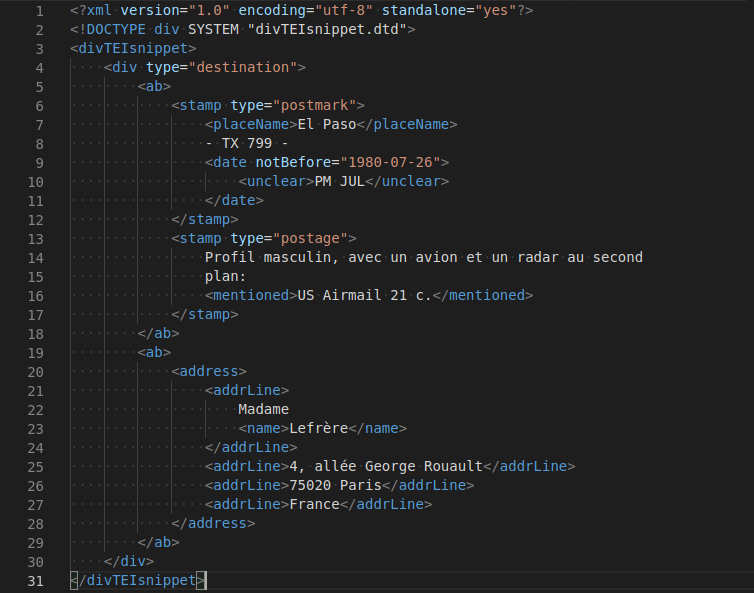
\includegraphics[width=.9\textwidth]{imgs/DivTEISnippet.png}
	\end{center}
	
\end{frame}

% sezione XML frame 02c
\begin{frame}
	\frametitle{TEI-XML}
	\framesubtitle{Motivazioni per adottare TEI}
	\addtocounter{nframe}{1}

	\begin{block}{Perché TEI}
		La Text Encoding Initiative (TEI) è un autorevole progetto internazionale, a cui afferiscono varie organizzazioni e università, il cui scopo è fornire agli studiosi di informatica umanistica uno strumento il più espressivo e flessibile possibile per rappresentare qualsiasi aspetto di interesse relativo alla risorsa testuale da rappresentare digitalmente.
	\end{block}

\end{frame}

% sezione XML frame 03
\begin{frame}
	\frametitle{Impiego di XML}
	\framesubtitle{Benefici}
	\addtocounter{nframe}{1}

	\begin{block}{Perché XML}
		\begin{itemize}
			\item separazione dei dati dall'applicativo di authoring/editing 
			\item separazione della rappresentazione dei dati dalla presentazione dei dati
			\item possibilità di trasformare i dati in qualsiasi altro formato compatibile
			\item leggibilità dei documenti XML da parte di esseri umani
		\end{itemize}

	\end{block}
	

\end{frame}

% sezione XML frame 03b
\begin{frame}
	\frametitle{Impiego di XML}
	\framesubtitle{Benefici}
	\addtocounter{nframe}{1}

	\begin{block}{Perché XML}
		\begin{itemize}
			\item standard w3c testuale, aperto, personalizzabile e liberamente utilizzabile
			\item semplicità di condivisione e scambio dati (interoperabilità e portabilità)
			\item adatto per codificare dati semistrutturati oltre che a dati strutturati
			\item validazione del documento attraverso spcificazioni formali
		\end{itemize}

	\end{block}
	

\end{frame}


% sezione XML frame 04
\begin{frame}
	\frametitle{Ecosistema XML}
	\framesubtitle{Le tecnologie XML per la definizione ed elaborazione di documenti XML}
	\addtocounter{nframe}{1}

	\begin{itemize}
		\item XSD: XML Schema Definition Language
		\item XPath: XML Path Language
		\item XSL: eXtensible Stylesheet Language
		\item XSL-T:  XSL – Transformations
		\item XSL-FO: XSL – Formatting Objects
		\item XQuery: XML Query Language for XML Databases
		\item XInclude: XML inclusion Language
		\item DTD: Document Type Definition Language
		\item RelaxNG: Regular Expression Language for XML (New Generation)
	\end{itemize}

\end{frame}


% sezione XML frame 05
\begin{frame}
	\frametitle{Linguaggio di marcatura XML}
	\framesubtitle{}
	\addtocounter{nframe}{1}

	\begin{block}{Perché XML}
		Adottando la tecnologia e il linguaggio XML abbiamo la possibilità di creare linguaggi di marcatura personalizzati e specifici per ogni esigenza e dominio.
	\end{block}

\end{frame}

\begin{frame}
	\frametitle{XML come linguaggio per la codifica di testi}
	\framesubtitle{}
	\addtocounter{nframe}{1}

	\begin{block}{Vantaggi}
		Attraverso XML è possibile strutturare i dati, gestire in modo nativo strutture gerarchiche, elaborare e presentare i dati con strumenti XML nativi, validare i tipi di strutture e i tipi di dati consentiti, gestire riferimenti incrociati tramite opportuni meccanismi di dereferenziazione, aggiungere e gestire annotazioni a vari livelli di granularità.
	\end{block}


\end{frame}
